\documentclass[11pt]{article}
\usepackage{amsmath,amssymb,amsmath,amsthm,amsfonts}
\usepackage{latexsym,graphicx}
\usepackage{fullpage,color}
\usepackage{url}
\usepackage[pdftex,bookmarks,colorlinks=true,citecolor=blue]{hyperref}
\usepackage{natbib}
\usepackage{graphicx,subfigure}
\usepackage{algorithm}
\usepackage{algorithmic}
\usepackage{listings}
\usepackage{xcolor}
\usepackage{framed}
\usepackage{color}

% \colorlet{shadecolor}{orange!15}
\colorlet{NextBlue}{orange!15!green!50!blue!75}

\numberwithin{equation}{section}

\pagestyle{plain}

\setlength{\oddsidemargin}{0in}
\setlength{\topmargin}{0in}
\setlength{\textwidth}{6.5in}
\setlength{\textheight}{8.5in}

\newtheorem{fact}{Fact}[section]
\newtheorem{question}{Question}[section]
\newtheorem{lemma}{Lemma}[section]
\newtheorem{theorem}[lemma]{Theorem}
\newtheorem{assumption}[lemma]{Assumption}
\newtheorem{corollary}[lemma]{Corollary}
\newtheorem{prop}[lemma]{Proposition}
\newtheorem{claim}{Claim}[section]
\newtheorem{remark}{Remark}[section]
\newtheorem{definition}{Definition}[section]
\newtheorem{prob}{Problem}[section]
\newtheorem{conjecture}{Conjecture}[section]
\newtheorem{property}{Property}[section]

\def\A{{\bf A}}
\def\a{{\bf a}}
\def\B{{\bf B}}
\def\bb{{\bf b}}
\def\C{{\bf C}}
\def\c{{\bf c}}
\def\D{{\bf D}}
\def\d{{\bf d}}
\def\E{{\bf E}}
\def\e{{\bf e}}
\def\F{{\bf F}}
\def\f{{\bf f}}
\def\g{{\bf g}}
\def\h{{\bf h}}
\def\G{{\bf G}}
\def\H{{\bf H}}
\def\I{{\bf I}}
\def\K{{\bf K}}
\def\k{{\bf k}}
\def\LL{{\bf L}}
\def\M{{\bf M}}
\def\m{{\bf m}}
\def\N{{\bf N}}
\def\n{{\bf n}}
\def\PP{{\bf P}}
\def\pp{{\bf p}}
\def\Q{{\bf Q}}
\def\q{{\bf q}}
\def\R{{\bf R}}
\def\rr{{\bf r}}
\def\S{{\bf S}}
\def\s{{\bf s}}
\def\T{{\bf T}}
\def\tt{{\bf t}}
\def\U{{\bf U}}
\def\u{{\bf u}}
\def\V{{\bf V}}
\def\v{{\bf v}}
\def\W{{\bf W}}
\def\w{{\bf w}}
\def\X{{\bf X}}
\def\x{{\bf x}}
\def\Y{{\bf Y}}
\def\y{{\bf y}}
\def\Z{{\bf Z}}
\def\z{{\bf z}}
\def\0{{\bf 0}}
\def\1{{\bf 1}}



\def\AM{{\mathcal A}}
\def\CM{{\mathcal C}}
\def\DM{{\mathcal D}}
\def\EM{{\mathcal E}}
\def\GM{{\mathcal G}}
\def\FM{{\mathcal F}}
\def\IM{{\mathcal I}}
\def\JM{{\mathcal J}}
\def\KM{{\mathcal K}}
\def\LM{{\mathcal L}}
\def\NM{{\mathcal N}}
\def\OM{{\mathcal O}}
\def\PM{{\mathcal P}}
\def\SM{{\mathcal S}}
\def\TM{{\mathcal T}}
\def\UM{{\mathcal U}}
\def\VM{{\mathcal V}}
\def\WM{{\mathcal W}}
\def\XM{{\mathcal X}}
\def\YM{{\mathcal Y}}
\def\RB{{\mathbb R}}
\def\RBmn{{\RB^{m\times n}}}
\def\EB{{\mathbb E}}
\def\PB{{\mathbb P}}

\def\TX{\tilde{\bf X}}
\def\TA{\tilde{\bf A}}
\def\tx{\tilde{\bf x}}
\def\ty{\tilde{\bf y}}
\def\TZ{\tilde{\bf Z}}
\def\tz{\tilde{\bf z}}
\def\hd{\hat{d}}
\def\HD{\hat{\bf D}}
\def\hx{\hat{\bf x}}
\def\nysA{{\tilde{\A}_c^{\textrm{nys}}}}

\def\alp{\mbox{\boldmath$\alpha$\unboldmath}}
\def\bet{\mbox{\boldmath$\beta$\unboldmath}}
\def\epsi{\mbox{\boldmath$\epsilon$\unboldmath}}
\def\etab{\mbox{\boldmath$\eta$\unboldmath}}
\def\ph{\mbox{\boldmath$\phi$\unboldmath}}
\def\pii{\mbox{\boldmath$\pi$\unboldmath}}
\def\Ph{\mbox{\boldmath$\Phi$\unboldmath}}
\def\Ps{\mbox{\boldmath$\Psi$\unboldmath}}
\def\ps{\mbox{\boldmath$\psi$\unboldmath}}
\def\tha{\mbox{\boldmath$\theta$\unboldmath}}
\def\Tha{\mbox{\boldmath$\Theta$\unboldmath}}
\def\muu{\mbox{\boldmath$\mu$\unboldmath}}
\def\Si{\mbox{\boldmath$\Sigma$\unboldmath}}
\def\si{\mbox{\boldmath$\sigma$\unboldmath}}
\def\Gam{\mbox{\boldmath$\Gamma$\unboldmath}}
\def\Lam{\mbox{\boldmath$\Lambda$\unboldmath}}
\def\De{\mbox{\boldmath$\Delta$\unboldmath}}
\def\Ome{\mbox{\boldmath$\Omega$\unboldmath}}
\def\Pii{\mbox{\boldmath$\Pi$\unboldmath}}
\def\varepsi{\mbox{\boldmath$\varepsilon$\unboldmath}}
\newcommand{\ti}[1]{\tilde{#1}}
\def\Ncal{\mathcal{N}}
\def\argmax{\mathop{\rm argmax}}
\def\argmin{\mathop{\rm argmin}}

\def\ALG{{\AM_{\textrm{col}}}}

\def\mean{\mathsf{mean}}
\def\std{\mathsf{std}}
\def\bias{\mathsf{bias}}
\def\var{\mathsf{var}}
\def\sgn{\mathsf{sgn}}
\def\tr{\mathsf{tr}}
\def\rk{\mathrm{rank}}
\def\nnz{\mathsf{nnz}}
\def\poly{\mathrm{poly}}
\def\diag{\mathsf{diag}}
\def\Diag{\mathsf{Diag}}
\def\const{\mathrm{Const}}
\def\st{\mathsf{s.t.}}
\def\vect{\mathsf{vec}}
\def\sech{\mathrm{sech}}
\def\sigmoid{\mathsf{sigmoid}}

\newcommand{\red}[1]{{\color{red}#1}}



\def\argmax{\mathop{\rm argmax}}
\def\argmin{\mathop{\rm argmin}}

\newenvironment{note}[1]{\medskip\noindent \textbf{#1:}}%
        {\medskip}


\newcommand{\etal}{{\em et al.}\ }
\newcommand{\assign}{\leftarrow}
\newcommand{\eps}{\epsilon}

\newcommand{\opt}{\textrm{\sc OPT}}
\newcommand{\script}[1]{\mathcal{#1}}
\newcommand{\ceil}[1]{\lceil #1 \rceil}
\newcommand{\floor}[1]{\lfloor #1 \rfloor}



\lstset{ %
extendedchars=false,            % Shutdown no-ASCII compatible
language=Python,                % choose the language of the code
xleftmargin=1em,
xrightmargin=1em,
basicstyle=\footnotesize,    % the size of the fonts that are used for the code
tabsize=3,                            % sets default tabsize to 3 spaces
numbers=left,                   % where to put the line-numbers
numberstyle=\tiny,              % the size of the fonts that are used for the line-numbers
stepnumber=1,                   % the step between two line-numbers. If it's 1 each line
                                % will be numbered
numbersep=5pt,                  % how far the line-numbers are from the code   %
keywordstyle=\color[rgb]{0,0,1},                % keywords
commentstyle=\color[rgb]{0.133,0.545,0.133},    % comments
stringstyle=\color[rgb]{0.627,0.126,0.941},      % strings
backgroundcolor=\color{white}, % choose the background color. You must add \usepackage{color}
showspaces=false,               % show spaces adding particular underscores
showstringspaces=false,         % underline spaces within strings
showtabs=false,                 % show tabs within strings adding particular underscores
frame=single,                 % adds a frame around the code
%captionpos=b,                   % sets the caption-position to bottom
breaklines=true,                % sets automatic line breaking
breakatwhitespace=false,        % sets if automatic breaks should only happen at whitespace
%title=\lstname,                 % show the filename of files included with \lstinputlisting;
%                                % also try caption instead of title
mathescape=true,escapechar=?    % escape to latex with ?..?
escapeinside={\%*}{*)},         % if you want to add a comment within your code
%columns=fixed,                  % nice spacing
%morestring=[m]',                % strings
%morekeywords={%,...},%          % if you want to add more keywords to the set
%    break,case,catch,continue,elseif,else,end,for,function,global,%
%    if,otherwise,persistent,return,switch,try,while,...},%
}


\begin{document}

%\setlength{\fboxrule}{.5mm}\setlength{\fboxsep}{1.2mm}
%\newlength{\boxlength}\setlength{\boxlength}{\textwidth}
%\addtolength{\boxlength}{-4mm}


\title{Poisoning attack review}

\author{\textbf{Mengjiao Zhang} \\ Stevens Institute of technology}

%\date{ }

\maketitle

% \begin{abstract}
% % This lecture note describes synchronous parallel accelerated gradient descent (AGD) for empirical risk minimization ERM.
% % We first describe AGD for solving ERM.
% % We then show how to parallelize AGD; in particular, we assume there is a central parameter server and the data are partitioned among the worker nodes.
% % We finally use Python to write a simulator that mimics synchronous parallel AGD.


% \end{abstract}




\section{Poisoning attack} \label{sec:optimization}

A poisoning attack happens when the adversary is able to inject bad data into your model’s training pool, and hence get it to learn something it shouldn’t. The most common result of a poisoning attack is that the model’s boundary shifts in some way.

\begin{figure}[!h]
	\centering
	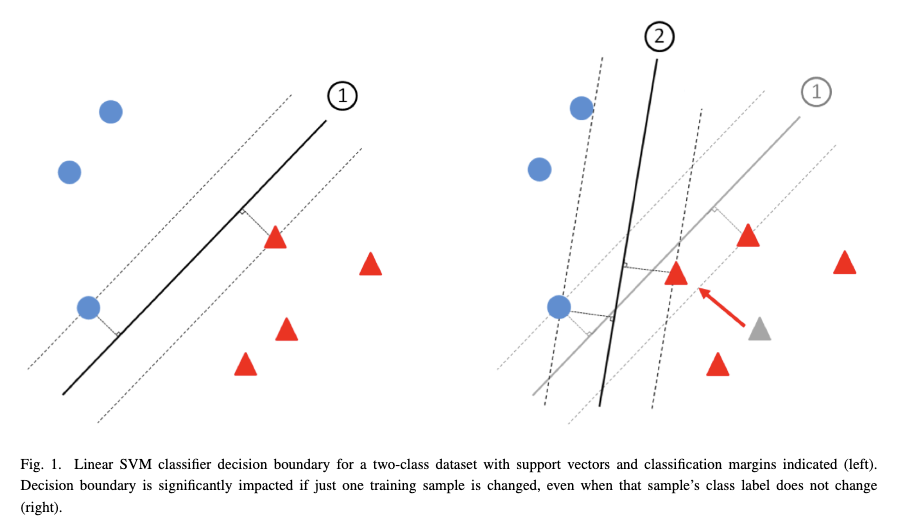
\includegraphics[width=16cm]{figures/poisoning_attack.png}
% 	\caption{Illustration of parallel AGD.}
	\label{fig:alg1}
\end{figure}

\colorbox{orange!15}{Two kind of poisoning attacks} \cite{poisoninga_ttack.org}:

\begin{enumerate}
    \item availability attack\\
    Inject so much bad data into the model that whatever boundary the model learns basically becomes useless.
    \item integrity attack {\color{blue} (also known as "backdoor attacks")}\\
    Leave the classifier functioning exactly like it should, with just one exception: a backdoor.
\end{enumerate}


\colorbox{orange!15}{Two types of adversaries:}

\begin{enumerate}
    \item WhiteBox {\color{blue}{(knows the internals of your model)}}
    \item BlackBox {\color{blue}{(doesn't)}}
\end{enumerate}

\colorbox{orange!15}{Levels of adversarial access(from most dangerous to least)}
\begin{itemize}
    \item Logic corruption\\
    The attacker can change the algorithm and the way it learns.
    \item Data manipulation
    Attacker can change/add to/remove from the training data.
    \begin{enumerate}
        \item manipulate labels.\\
        Draw new labels for a part of the training pool or try to optimize them to cause maximum disruption.
        \item manipulate the input(more sophisticated).\\
        Perturb the input to shift the classification boundary, change cluster distance, or add an invisible watermark that can later be used to "backdoor" into the model.
    \end{enumerate}
    \item data injection\\
    Limited to addition. Inject new data into the training pool.
    \item Transfer learning\\
    As the network goes through its second training, its original memories (including the poison) get diluted.
\end{itemize}

% \begin{figure}[!h]
% 	\centering
% 	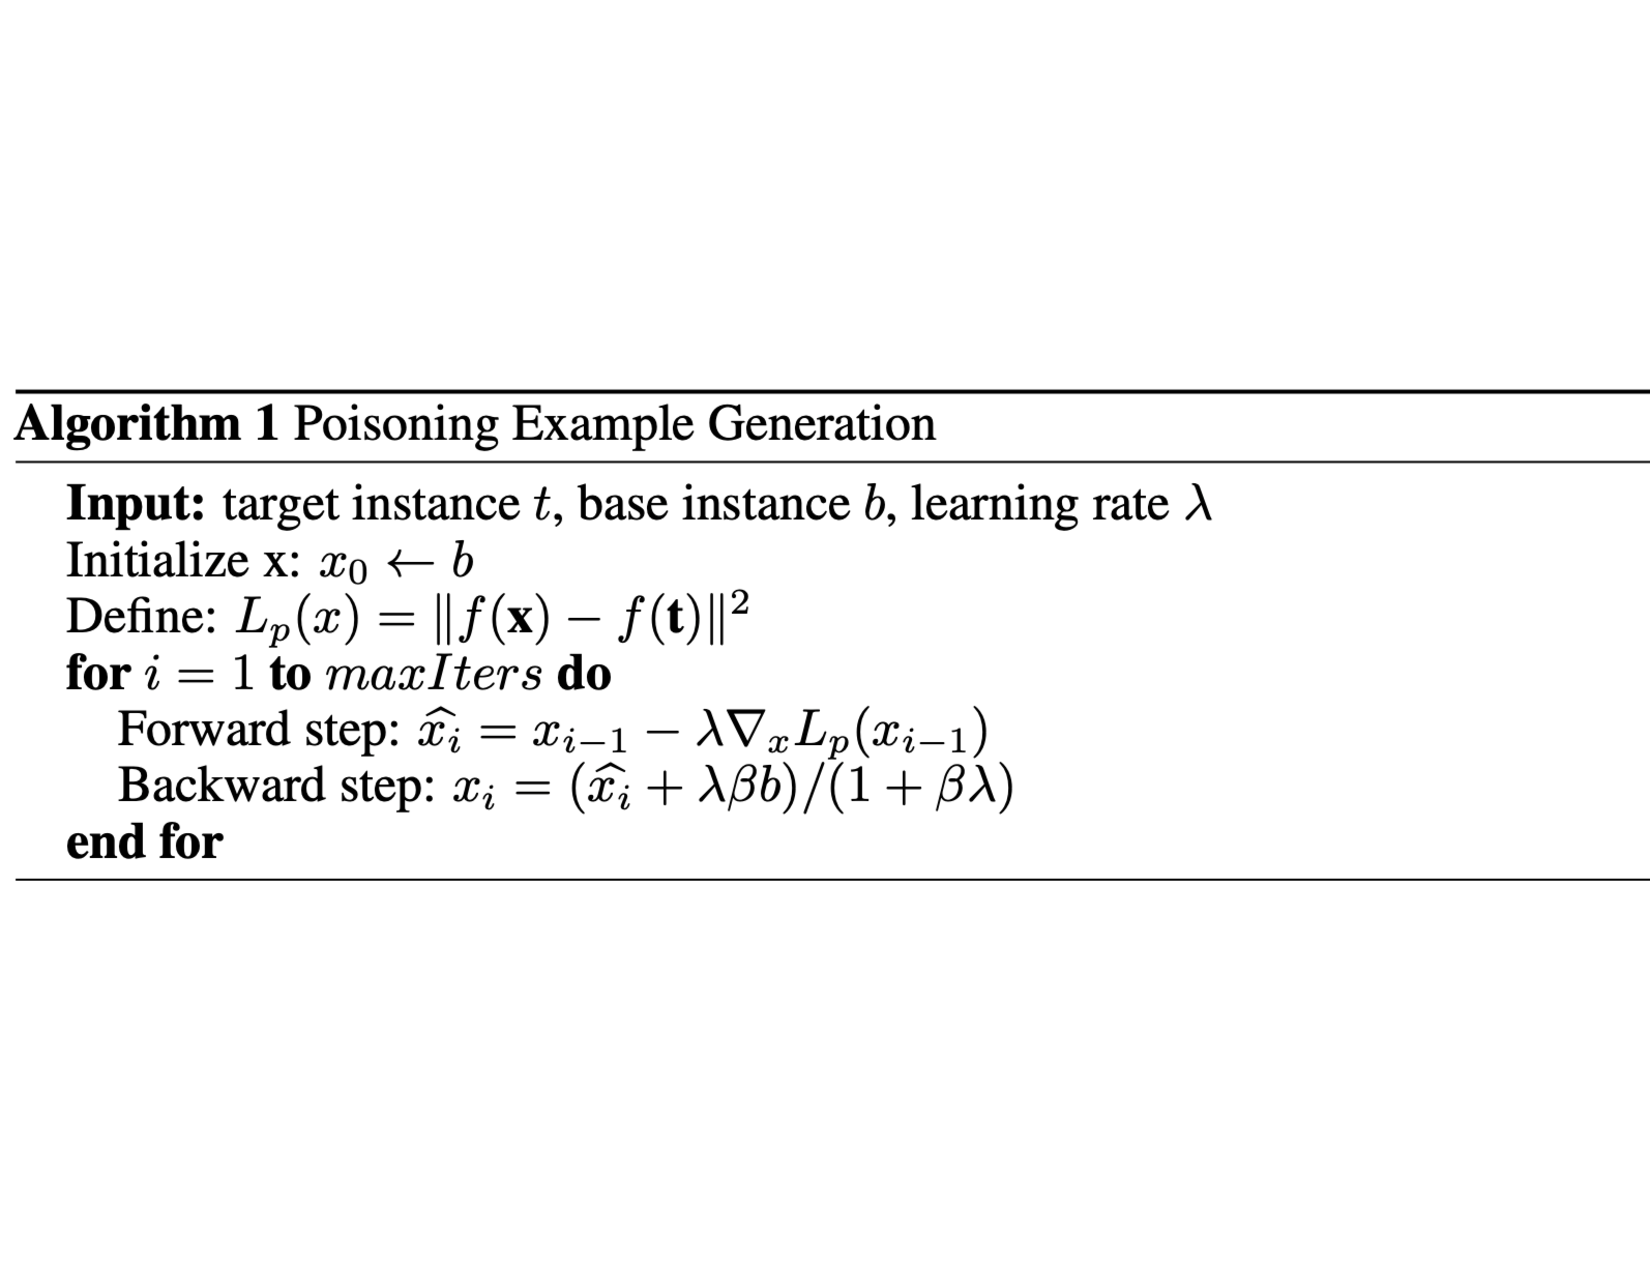
\includegraphics[width=17cm]{figures/alg1.pdf}
% % 	\caption{Illustration of parallel AGD.}
% 	\label{fig:alg1}
% \end{figure}


\section{Defenses Against Data poisoning}

\colorbox{orange!15}{\textbf{Most common type of defense}}\\

{\color{red} Outlier detection}, also knows as {\color{red} "data sanitization"} and {\color{red} "anomaly detection"}.

\textbf{The idea:}

When poisoning a machine learning system the attacker is by definition injecting something into the training pool that is \textit{very} different to what it should include.

\begin{figure}[!h]
	\centering
	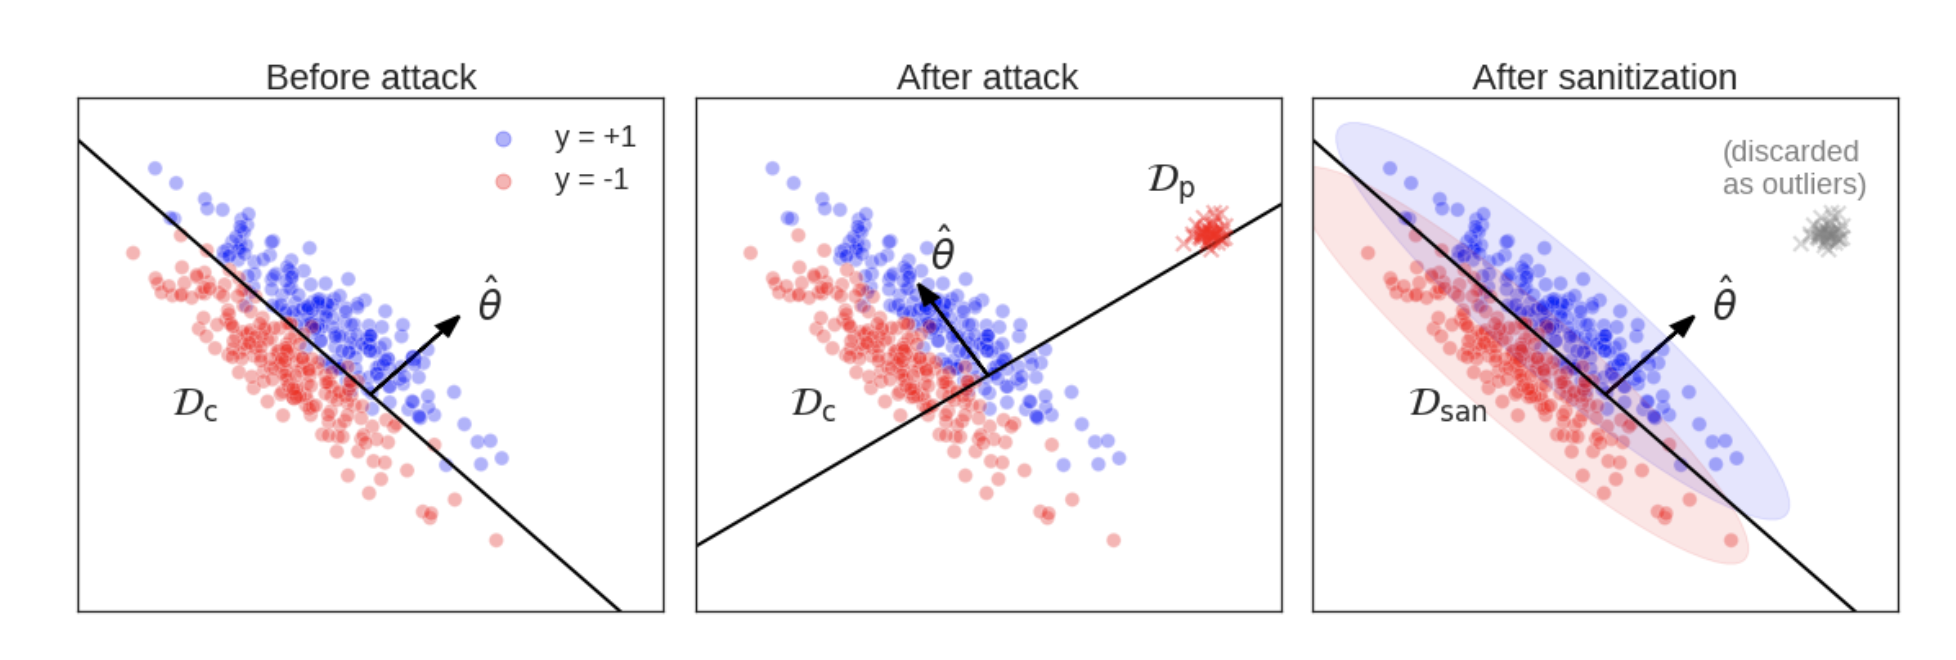
\includegraphics[width=16cm]{figures/poisoning_injection_outliers.png}
% 	\caption{Illustration of parallel AGD.}
	\label{fig:outliers}
\end{figure}

\textbf{Challenge:}

quantifying "\textit{very}". 

Sometimes the poison injected is from a different data distribution and can be easily isolated(\figureautorefname{\ref{fig:outliers}}).

In other cases, the poison points are generated from distributions that are very similar to the true data distribution(called "inliers"), but that still successfully mislead the model.

Another scenario where outlier detection breaks down:poison was injected before filtering rules were created.

\textbf{Micromodels defense.}

Training classifiers on non-overlapping epoches of the training set(micromodels) and evaluate them on the training set.

\colorbox{orange!15}{\textbf{The second most common type of defense:}}

analyze the impact of newly added training samples on \textbf{model's accuracy}.

\colorbox{orange!15}{Some other interesting defenses:}
\begin{itemize}
    \item STRIP = intentionally perturb the inputs and observe variance in predictions vs unperturbed. If not enough variance = malicious.
    \item Human in the loop = it’s known that poisoning outliers leads to bigger boundary shifts, so why not focus human (presumably security analyst) attention on only such cases?
    \item TRIM = model learns in iterations from “trimmed” versions of MSEs (regression).
\end{itemize}


\bibliographystyle{plain}

%\markboth{\bibname}{\bibname}
% \bibliography{bib/decentralized,bib/distributed,bib/system}
\bibliography{bib/decentralized,bib/distributed,bib/system,bib/poison}

\end{document}
